\documentclass[a4paper]{article}
\usepackage{ucs}
\usepackage[utf8x]{inputenc}
\usepackage{changepage}
\usepackage{graphicx}
\usepackage{amsmath}
\usepackage{gensymb}
\usepackage{amssymb}
\usepackage{enumerate}
\usepackage{tabularx}
\usepackage{lipsum}
\usepackage{amsthm}
\usepackage{thmtools}
\usepackage{xcolor}



%\documentclass[jou]{apa6}
%\usepackage[american]{babel}

%\usepackage{csquotes}
%\usepackage[style=apa,sortcites=true,sorting=nyt,backend=biber]{biblatex}
%\DeclareLanguageMapping{american}{american-apa}
%\addbibresource{bibliography.bib}


%%%%%%%%%%%%%%%%%%%%%%%%%%%%%%%%%%%%%%%%
%% Discrete Structures
%% The start of RBS stuff
%%%%%%%%%%%%%%%%%%%%%%%%%%%%%%%%%%%%%%%%

% Working internal and external links in PDF
\usepackage{hyperref}
% Extra math symbols in LaTeX
\usepackage{amsmath}
\usepackage{gensymb}
\usepackage{amssymb}
% Enumerations with (a), (b), etc.
\usepackage{enumerate}
\usepackage[framemethod=TikZ]{mdframed}
\usepackage{xcolor}

\let\OLDitemize\itemize
\renewcommand\itemize{\OLDitemize\addtolength{\itemsep}{-6pt}}

\usepackage{etoolbox}
\makeatletter
\preto{\@verbatim}{\topsep=3pt \partopsep=3pt }
\makeatother

% These sizes redefine APA for A4 paper size
\oddsidemargin 0.0in
\evensidemargin 0.0in
\textwidth 6.27in
\headheight 1.0in
\topmargin -24pt
\headheight 12pt
\headsep 12pt
\textheight 9.19in

\setlength{\parindent}{0pt}
\setlength{\columnsep}{1cm}



\begin{document}

\twocolumn


\begin{center}
{\Large Beigu eksāmens}
\end{center}


{\bf Termiņš:} 2020.gada 21.decembris, līdz vakaram\\
{\bf Iesniegšanas veids:} E-studiju vide.

\vspace{5pt}
{\bf 1.uzdevums (Rabina-Karpa algoritms)}\\
RNA vīrusu genomu virknes pieraksta ar burtiem {\tt A,C,G,U}.
Mums dots garš teksts $T[0..n-1]$ garumā $n$, kas pierakstīts ar 
šiem burtiem. Un tajā jāmeklē paraudziņš, kas norāda uz 
vīrusa mutāciju: $\textcolor{blue}{\mathtt{GUCAGA}}$. 

\vspace{5pt}
{\bf (A)} Alise aizstāj šos četrus RNA genoma burtus ar to skaitliskajām 
vērtībām: $\mathtt{A} = 0$, $\mathtt{C} = 1$, $\mathtt{G} = 2$, 
$\mathtt{U} = 3$. Tā kā vīrusam-mutantam atbilstošais paraugs ir garumā $6$ simboli, 
arī meklējamais logs ir tikpat garš. Katrai nobīdei $s \in [0,n-6]$ 
aplūkojam pārbaudāmajā tekstā $T$ kaut kādus sešus pēc kārtas esošus simbolus 
$T[s]$, $T[s+1]$, $T[s+2]$, $T[s+3]$, $T[s+4]$, $T[s+5]$. 
Visi tie ir no kopas $\{ 0,1,2,3 \}$. Rēķinām hešfunkciju: 
$$h_A(T[s..s+5]) = \left( \sum\limits_{k=0}^{5} T[s+k] \cdot x^k \right)\;(\text{mod}\,p),$$
kur polinoma mainīgais $x = 4$, bet pirmskaitlis $p = 1093$
(t.i. pirmskaitlis, kurš nedaudz lielāks par $2^5 = 1024$).\\


Atrast, cik daudzām $6$-burtu kombinācijām $w$, kas uzrakstāmas ar 
alfabētu {\tt A,C,G,U} būs spēkā kolīzija ar meklējamo paraugu:
$$h_A(w) = h_A(\mathtt{GUCAGA}).$$



\vspace{5pt}
{\bf (B)}
Bobs izmanto citu hešfunkciju: Rabina-Karpa algoritma 
autora ieteikto Rabina digitālnospiedumu 
(Rabin fingerprint), sk. \url{https://bit.ly/2LUwuxo}. 
Viņš iekodē $6$ pēc kārtas sekojošus RNA alfabēta burtus no 
meklējamā teksta $T$ par $12$ bitu virknīti
($\mathtt{A} = 00$, $\mathtt{C} = 01$, $\mathtt{G} = 10$, $\mathtt{U} = 11$). 
Tad pieraksta to kā 11.pakāpes polinomu ar $12$ koeficientiem: 
$$f(x) = m_0 + m_1 x + \ldots + m_{11} x^{11},$$
kur (atšķirībā no Alises hešfunkcijas $h_A$) pirmais burts dod polinomā jaunākos 
locekļus, bet pēdējais burts dod vecākos. 
Pēc tam Bobs dala iegūto 11.pakāpes polinomu ar nereducējamu 
10.pakāpes polinomu $Q(x) = x^{10} + x^3 + 1$ koeficientu laukā $GF(2)$
(t.i. pēc pirmskaitļa $2$ moduļa) un iegūst atlikumu 
$R(x)$, kas ir Boba hešfunkcijas vērtība. 

Piemēram, mutantu vīrusa raksturīgajai virknītei
$\textcolor{blue}{\mathtt{GUCAGA}}$ atbilst bitu virknīte 
$\textcolor{blue}{\mathtt{10.11.01.00.10.00}}$. No tās rodas 
polinoms:
$$P(x) = 1 + 1x^2 + 1x^3 + 1x^5 + 1x^8.$$
Šī polinoma dalījums ar $x^{10} + x^3 + 1$ dod atlikumu, kas ir viņš pats
(bet tiek jau aplūkots kā 9.pakāpes polinoms, nevis 11.pakāpes polinoms), 
t.i. Boba hešfunkcija:
$$h_B(\textcolor{blue}{\mathtt{GUCAGA}}) = \mathtt{10.11.01.00.10}.$$
Kā redzam, pēc hešfunkcijas pēdējie divi biti ``pazūd''. 

Atrast, cik daudzām $6$-burtu kombinācijām $w$, kas uzrakstāmas ar 
alfabētu {\tt A,C,G,U} būs spēkā kolīzija ar meklējamo paraugu:
$$h_B(w) = h_B(\mathtt{GUCAGA}).$$

\vspace{5pt}
{\footnotesize
{\em Piezīme.} Boba gadījumā (atšķirībā no Alises) polinomu $P(x)$ izmanto nevis, lai aprēķinātu 
polinoma vērtību kādai mainīgā $x$ vērtībai, bet gan kā simbolisku pierakstu, 
lai iegūtu polinomu dalījuma atlikumu. Lai redzētu, kā darbojas polinomu aritmētika 
pēc $2$ moduļa, minēsim vēl vienu Boba hešfunkcijas aprēķina piemēru.

Ar Boba hešfunkciju iekodējamais $6$-burtu vārds $w = \textcolor{blue}{\mathtt{CAGUAU}}$. 
Pārveidojam par bitu virknīti: $\mathtt{01.00.10.11.00.11}$ un uzrakstām 
sākotnējo 11.pakāpes polinomu: 
$$P(x) = $$
$$=0 + 1x^1 + 0x^2 + 0x^3 + 1x^4 + 0x^5 + 1x^6 + 1x^7 + 0x^8 + 0x^9 + 1x^{10} + 1x^{11}=$$
$$ = x + x^4 + x^6 + x^7 + x^{10} + x^{11} = $$
$$ = x^{11} + x^{10} + x^7 + x^6 + x^4 + x.$$
Lai atrastu atlikumu, dalot ar $Q(x) = x^{10} + x^3 + 1$, vispirms atrodam 
$P(x) - x\cdot{}Q(x)$, lai atbrīvotos no saskaitāmā $x^{11}$:
$$P(x) - x\cdot{}Q(x) = $$
$$=\left( x^{11} + x^{10} + x^7 + x^6 + x^4 + x \right) - 
x \cdot \left( x^{10} + x^3 + 1 \right) = $$
$$=x^{11} + x^{10} + x^7 + x^6 + x^4 + x - x^{11} - x^4 - x = $$
$$=x^{10} + x^7 + x^6.$$
Tagad atņemam $Q(x)$, lai atbrīvotos arī no saskaitāmā $x^{10}$: 
$$\left( x^{10} + x^7 + x^6 \right) - \left( x^{10} + x^3 + 1 \right)=$$
$$= x^7 + x^6 - x^3 - 1 = x^7 + x^6 + x^3 + 1.$$
Šajos pārveidojumos izmantojām, ka $-1 \equiv 1$ (mod $2$). 
Tātad $R(x) = x^7 + x^6 + x^3 + 1$ arī ir meklētais atlikums. 

Pārrakstām to kā 10-bitu virknīti, sākot no jaunākā koeficienta:
$$R(x) = 1 + x^3 + x^6 + x^7 = \sum_{i=0}^{9} a_i \cdot x^i.$$
Iegūstam $(a_0,\ldots,a_{9}) = (1,0,0,1,0,0,1,1,0,0)$ un tātad
Boba hešfunkcija 
$$h_B(\textcolor{blue}{\mathtt{CAGUAU}}) = \mathtt{10.01.00.11.00}.$$
Kā redzam, visos šajos pārveidojumos mums nav jāievieto konkrētas $x$ vērtības; 
Boba gadījumā $x$ ir tikai simbolisks apzīmējums, kas palīdz 
veikt polinomu dalīšanu ar atlikumu. Mūs interesējošais rezultāts pats ir 
polinoms $R(x)$.
}


\vspace{5pt}
{\bf (C)} Alises un Boba hešfunkcijām atrast varbūtību, ka 
Rabina-Karpa algoritms sastaps meklējamā tekstā kolīziju, ja meklējamais 
$6$ burtu paraudziņš $P$ ar vienādu varbūtību ir 
jebkura $6$ burtu RNA virkne, bet teksts $T$ ir nejauši veidots un garš. 


%\vspace{5pt}
%{\bf (B)} Bobs iekodē RNA genoma burtus kā bitu virknīti, apzīmējot
%$\mathtt{A} = 00$, $\mathtt{C} = 01$, $\mathtt{G} = 10$, 
%$\mathtt{U} = 11$.
%Viņa gadījumā arī teksts $T$ iekodējas divreiz garāks (tā garums ir 
%$2n$ biti, jo katru RNA genoma burtu tagad apzīmē $2$ biti). 
%Un Bobs tālāk veido Rabina digitālnospiedumu (sk. \url{


% https://stackoverflow.com/questions/7043778/longest-palindrome-in-a-string-using-suffix-tree
% https://www.geeksforgeeks.org/longest-palindromic-subsequence-dp-12/


\vspace{20pt}
{\bf 2.uzdevums (Garākais palindroms).}\\

Mūsu uzdevums ir atrast garāko substringu do\-ta\-jā stringā $P$, kas vienlaikus būtu 
palindroms (lasītos no abiem galiem vienādi). Ja šādu garāko palindromu ir vairāki, 
pietiek atrast vienu no tiem.
Piemēram, vārdā $\textcolor{blue}{\mathtt{BANANA}}$ garākais palindroms ir $\mathtt{ANANA}$, 
vārdā $\textcolor{blue}{\mathtt{ANNA}}$ garākais palindroms ir pats $\mathtt{ANNA}$, 
vārdā $\textcolor{blue}{\mathtt{ABRAKADABRA}}$ garākais palindroms ir $\mathtt{AKA}$, 
bet vārdā  $\textcolor{blue}{\mathtt{ABCD}}$ tas ir viena burta strings, piemēram, $\mathtt{A}$.

\vspace{5pt}
{\bf (A)} Aplūkosim naivo algoritmu, kas apskata visus iespējamos dotā stringa $P$ apakšstringus; 
katram no tiem pārbauda, vai tas ir palindroms. 
Kāda ir šī algoritma laika sarežģītība $O(f(n))$? (Šeit $n$ - ievades stringa garums.)



\vspace{5pt}
{\bf (B)}
Kāds programmētājs piedāvā lietot Ukkonena algoritmu un izveidot sufiksu
koku, kurš uzbūvēts no sekojošu divu vārdu sufiksiem:\\
$P = \textcolor{blue}{\mathtt{BANANA\$}}$, 
$P_{rev} = \textcolor{green}{\mathtt{ANANAB\#}}$.\\
$P_{rev}$ ir $P$ uzrakstīts no otra gala un izmantoti divi dažādi beigu marķieri 
$\texttt{\$}$ (sākotnējam stringam) un $\texttt{\#}$ (reversajam stringam). 

Izveidotajā kokā atrodam visdziļāk esošo 
iekšējo virsotni, zem kuras ir gan zilas, gan zaļas lapas (t.i. kas var beigties 
gan ar $\texttt{\#}$, gan ar $\texttt{\$}$).
Mūsu gadījumā šī virsotne ir $\mathtt{ANANA}$ (apvilkts ar aplīti Attēlā~\ref{fig:banana-suffix-tree}.
Tas ir arī garākais palindroms, kas ietilpst vārdā $\mathtt{BANANA}$

\vspace{5pt} 
{\em Piezīme.} Virsotnes $v$ dziļumu sufiksu kokā definē kā burtu skaitu, kas jānolasa, lai 
no sufiksu koka saknes tiktu līdz $v$.


\begin{figure}[!htb]
\center{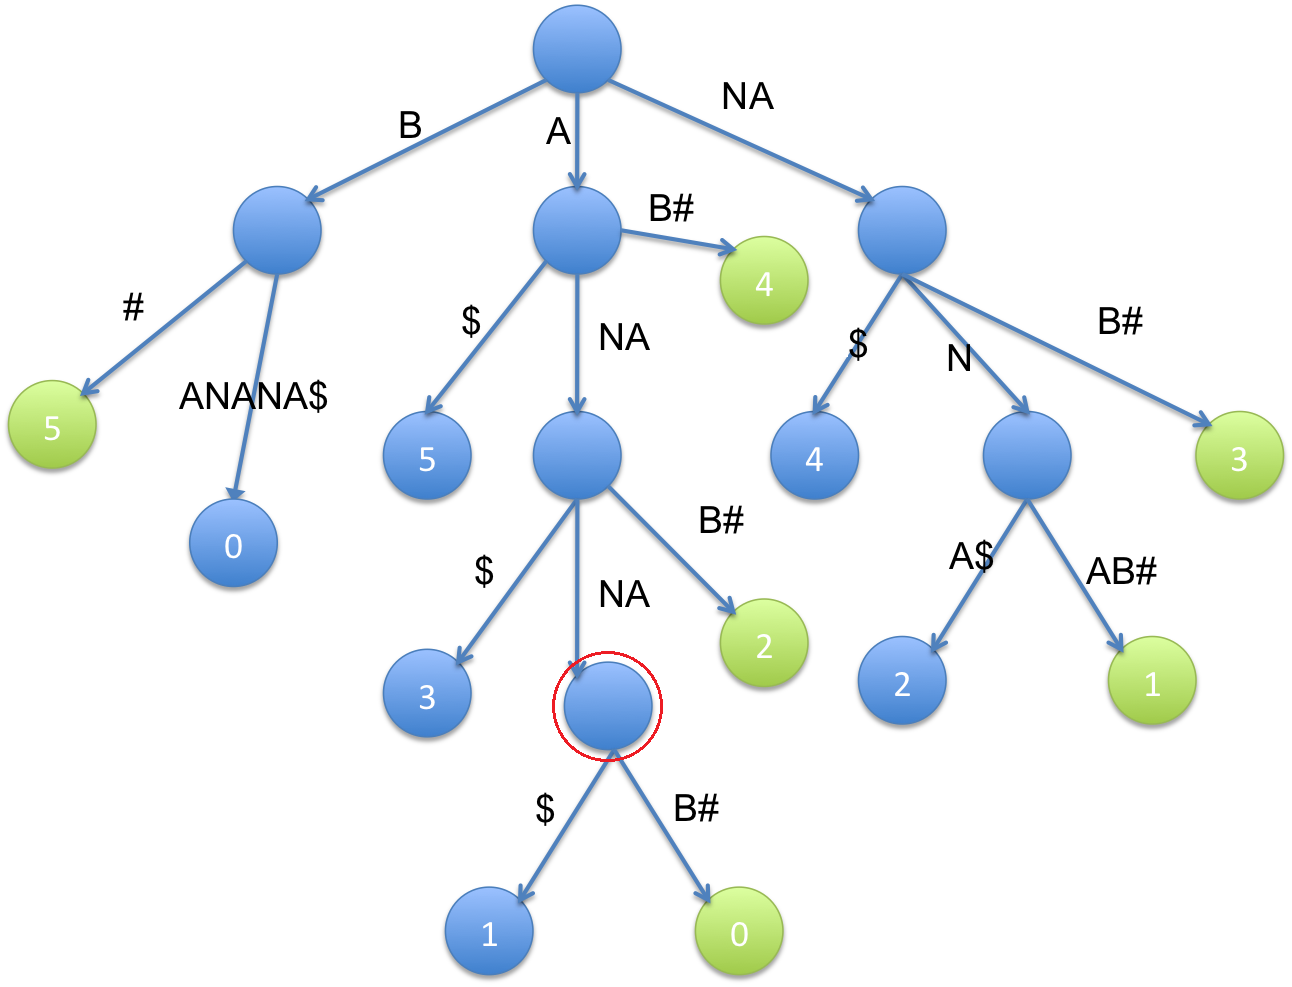
\includegraphics[width=2.6in]{fall2020-final/banana-suffix-tree.png}}
\caption{\label{fig:banana-suffix-tree} Sufiksu koks 2 stringiem.}
\end{figure}

Pēc Attēla~\ref{fig:banana-suffix-tree} parauga izveidot un uzzīmēt kopīgu sufiksu koku stringiem\\
$P = \textcolor{blue}{\mathtt{KLIBIBIKLI\$}}$ un 
$P_{rev} = \textcolor{green}{\mathtt{ILKIBIBILK\#}}$. 


\vspace{5pt}
{\bf (C)} Atrast pretpiemēru iepriekšējā punktā aprakstītajai
palindromu meklēšanas metodei, kur $P$ un $P_{rev}$ kopīgajā sufiksu kokā
atrastā dziļākā iek\-šē\-jā virsotne, 
kuru var pabeigt gan kā stringa $P$ sufiksu, gan kā $P_{rev}$ sufiksu, nemaz nav palindroms
(vai arī nav visgarākais starp palindromiem, kurš ietilpst stringā $P$).  

\vspace{5pt}
{\bf (D)} Aprakstīt tādu palindromu meklēšanas me\-to\-di, kas arī 
var izmantot Attēlam~\ref{fig:banana-suffix-tree} līdzīgu 
$P$ un $P_{rev}$ kopīgo sufiksu koku, bet tam nemēdz būt pretpiemēri (kā {\bf (C)}). 
Atrast Jūsu palindromu meklēšanas metodei laika sarežģītību.
(Vēlams, lai tā strādātu ātrāk nekā algoritms no {\bf (A)}.)



\vspace{20pt}
{\bf 3.uzdevums (Primārais un duālais LP)}

Dots primārais LP uzdevums: Maksimizēt $z = 2x_1 + 5x_2$, 
kur $3x_1 + 7x_2 = 12$ un $x_1,x_2 \geq 0$.

\vspace{5pt}
{\bf (A)} Kāds ir primārā LP mērķfunkcijas $2x_1 + 5x_2$ maksimums, un pie kuriem $x_i$ to var sasniegt.

\vspace{5pt}
{\bf (B)} Formulēt dotajam primārajam duālo LP uzdevumu.

\vspace{5pt}
{\bf (C)} 
Atrast duālā uzdevuma mērķfunkcijas minimumu un kādām mainīgo vērtībām to sasniedz.





\end{document}

